\section{Ablation}
\label{sec:ablation}

Table~\ref{tab:ablation} lists the \ablMutants{} defects planted in the released engine and the layers that detect each, and Figure~\ref{fig:ablation-matrix} draws the same matrix. The engine as released passes all five layers (\ablFalseAlarms{} false alarms), and passes them again after the last defect is removed; a false alarm at either point would have stopped the run. A layer detects a defect only when one of its checks fails. An exception raised while a layer runs, such as an exhausted memory, is a failed run: the script runs the layer again and, if the exception persists, stops without writing a result, and in the committed run a layer was run again after an exception \ablRetriesCommitted{} times, and the committed matrix was reproduced cell for cell by \ablReproduced{} of \ablReruns{} further runs of the script (Section~\ref{sec:reproducibility}). The rule matters because an earlier version of the script recorded an exception as a detection; on a loaded machine a rerun of that version, by a reader other than the writer, recorded four detections that were memory errors, in layers $C$ and $E$, and with them layer $D$ had no unique detection and Hypothesis~H8 failed. Ten of the defects change a result of the engine; two (a different seed and a different chunk size of the sampler) change the sample path and not its distribution, and are labelled equivalent in the table.

\begin{table}[htbp]
\centering
\small
\caption{Defects planted one at a time in the released engine and the verification layers that detect each: A analytic anchors, B published vectors and the ECB transcription, C regeneration of the committed rung, D known-truth simulator, E cross-implementation; x marks a detection.}
\label{tab:ablation}
\begin{tabular}{lp{6.4cm}cccccc}
\toprule
Id & Defect planted in the engine & Equivalent & A & B & C & D & E \\
\midrule
P01 & granularity delta scaled by 1.02 & no & . & x & . & . & . \\
P02 & large-portfolio distribution function with the correlation scaled by 1.05 & no & x & . & . & . & . \\
P03 & copula sampler drawn with the next seed (statistically equivalent) & yes & . & . & x & . & . \\
P04 & copula loadings scaled by 0.97 (correlation 6 percent low) & no & . & . & x & . & . \\
P05 & CreditRisk+ recursion shifted by one loss unit & no & x & . & . & . & x \\
P06 & Jeffreys prior Beta(1, 1) in place of Beta(1/2, 1/2) & no & . & x & . & . & . \\
P07 & concentration statistic with sqrt(K) in place of sqrt(K-1) & no & . & x & . & . & . \\
P08 & flattener long coefficient 0.65 in place of 0.60 & no & . & x & . & . & x \\
P09 & present value with annual compounding in place of continuous & no & . & . & . & . & x \\
P10 & maximum-likelihood correlation scaled by 0.7 & no & . & . & . & x & . \\
P11 & large-portfolio capital scaled by 1.01 & no & x & . & . & . & . \\
P12 & copula sampler ignores the committed chunk size (statistically equivalent) & yes & . & . & x & . & . \\
 & Detections of the defects that change a result &  & 3 & 4 & 1 & 1 & 3 \\
\bottomrule
\end{tabular}
\end{table}


\begin{figure}[htbp]
\centering
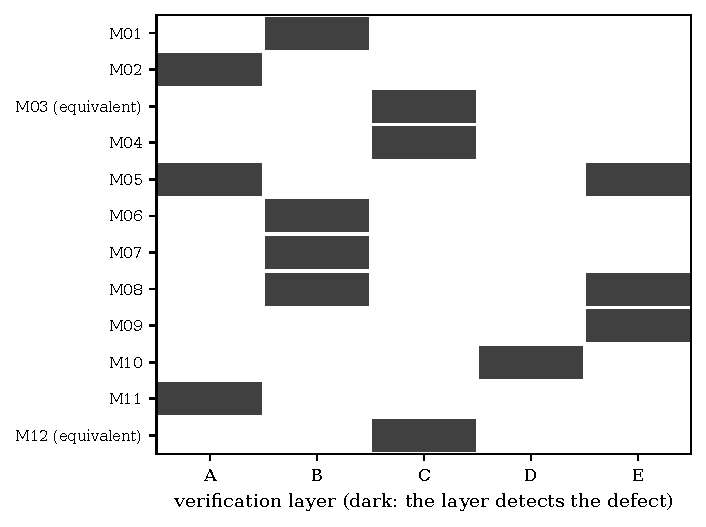
\includegraphics[width=0.62\textwidth]{ablation-matrix}
\caption{Detection matrix of the \ablMutants{} planted defects (rows) by the five verification layers (columns): a dark cell means the layer detects the defect; the two defects labelled equivalent change the sample path of the sampler and not its distribution.}
\label{fig:ablation-matrix}
\end{figure}

\subsection{What each layer contributes}

Layer A, the analytic anchors, detects \ablAReal{} of the \ablReal{} defects that change a result. It finds the correlation scaled in the large-portfolio distribution function (found by: \ablDetTwo{}), the recursion shifted by one loss unit (\ablDetFive{}) and the large-portfolio capital scaled by one per cent (\ablDetEleven{}). Layer B, the published vectors and the ECB transcription, detects \ablBReal{}: the granularity factor scaled by 1.02 (\ablDetOne{}), the Jeffreys prior changed from one half to one (\ablDetSix{}), the concentration statistic with the wrong square root (\ablDetSeven{}) and the flattener coefficient (\ablDetEight{}); none of these four moves a quantity that the anchors evaluate. Layer C, the regeneration of the committed rung, detects \ablCAll{} defects of the twelve, which are the two defects that change the sample path without changing the distribution and the loading defect (\ablDetFour{}); of the real defects it detects \ablCReal{}. Layer D, the known-truth simulator, detects \ablDReal{}: the maximum-likelihood correlation scaled by 0.7 (\ablDetTen{}), which no arithmetic check evaluates. Layer E, the cross-implementation checks, detects \ablEReal{}: the recursion shift (\ablDetFive{}), the flattener coefficient (\ablDetEight{}) and the annual compounding that replaces the continuous one (\ablDetNine{}); the last is found by no other layer.

\subsection{The unique detections and the equivalent defects}

\ablAny{} of the \ablReal{} real defects are detected by at least one layer, \ablOnly{} by exactly one, and \ablNone{} by none. Each layer detects a real defect that no other layer detects: the distribution function and the capital scaled by a constant for the anchors, the granularity, the prior and the concentration square root for the vectors, the loading defect for the regeneration, the biased estimator for the known-truth simulator and the compounding rule for the cross-implementation layer. Hypothesis~H8 therefore \ablHEight{}: \ablLayersWithUnique{} of the five layers have a unique detection (layer $A$ \ablAUnique{}, $B$ \ablBUnique{}, $C$ \ablCUnique{}, $D$ \ablDUnique{} and $E$ \ablEUnique{}). The hypothesis measures how far the check sets cover the engine: each unique detection follows from the engine function that the layer exercises and that no other layer calls (Section~\ref{sec:limitations}), and only two defects are seen by two layers. The two equivalent defects are detected by layer C and by no other, \ablCEquiv{} of \ablEquiv{}: the regeneration check is a regression check, since it signals any change in the sequence of random numbers that the committed result was generated from, whether or not the change matters to the engine's statistics, and a signal from it that no other layer confirms calls for a decision about whether the change is a defect and not for a fix.

\subsection{The loading defect against the resolution of the cross-implementation layer}

The one real defect that only the regeneration found is the scaling of the copula loadings by \effLoadingFactor{}, which lowers the asset correlation by \effCorrPct{} per cent. At the size of the main comparison it moves the 99\,\% value at risk of the engine by \effChangeVarNinetyNine{}\,\%, the 99\,\% expected shortfall by \effChangeEsNinetyNine{}\,\%, the 99.9\,\% value at risk by \effChangeVarNinetyNineNine{}\,\% and the 99.9\,\% expected shortfall by \effChangeEsNinetyNineNine{}\,\% (mean over \effReps{} seeds of \effScen{} scenarios, against the engine without the defect). The cross-implementation layer compares three runs of 40,000 scenarios for each route on the 99\,\% value at risk and rejects at four standard errors, so by Proposition~\ref{prop:power}, with $c=4$ and the run-to-run error scaled with the square root of the number of scenarios and runs, its minimum detectable shift at a power of $0.8$ is \effMddVarNinetyNine{}\,\% of the 99\,\% value at risk; a Student distribution with four degrees of freedom would make it larger still. The shift of the defect, \effChangeVarNinetyNine{}\,\%, is below that resolution, so the layer as run cannot detect it, and it does not.

At the size of the main comparison the minimum detectable shifts at the cutoff $c=3$ of Hypothesis~H3 are \mcMddVarNinetyNine{}, \mcMddEsNinetyNine{}, \mcMddVarNinetyNineNine{} and \mcMddEsNinetyNineNine{}\,\% of the four measures. The defect was run at that size: \fsReps{} runs of \fsScen{} scenarios of the defective engine, compared with the stored runs of the independent simulator of Section~\ref{sec:results}. The shifts from the independent simulator are \fsShiftVarNinetyNine{}, \fsShiftEsNinetyNine{}, \fsShiftVarNinetyNineNine{} and \fsShiftEsNinetyNineNine{}\,\%, and $z=\fsZVarNinetyNine{}$, $\fsZEsNinetyNine{}$, $\fsZVarNinetyNineNine{}$ and $\fsZEsNinetyNineNine{}$ for the 99\,\% value at risk, the 99\,\% expected shortfall, the 99.9\,\% value at risk and the 99.9\,\% expected shortfall (defective engine minus independent simulator). The full-size comparison therefore rejects the engine on \fsFlagged{} of the four measures by the criterion $|z|\le3$ of Hypothesis~H3 and misses it on the 99.9\,\% expected shortfall, whose minimum detectable shift is close to the shift the defect produces there. The conclusion is not that the independent simulator is weak, but that its resolution is a number that Proposition~\ref{prop:power} computes, that a validator can choose by the number of runs and of scenarios, and that one defect at one size illustrates it and does not map it.
